

\documentclass[colorlinks=true,pdfstartview=FitV,linkcolor=blue,
            citecolor=red,urlcolor=magenta]{ligodoc}

\usepackage{graphicx}
\usepackage{amssymb}
\usepackage{amsmath}
\usepackage{longtable}
\usepackage{rotating}
\usepackage[usenames,dvipsnames]{color}
\usepackage{fancyhdr}
\usepackage{subfigure}
\usepackage{hyperref}
\ligodccnumber{T}{11}{XXXXX}{}{vX}% \ligodistribution{AIC, ISC}


\title{Devoloping Phase Map of Cavity Mirrors using Laser Mode Spectroscopy }

\author{Keerthana S Nair
\newline{Mentors: Gautam Venugopal, Koji Arai and Rana Adhikari}}

\begin{document}


\section{Introduction} 
\subsection{Gravitational Waves}
Einstein's general theory of relativity explains gravity as a distortion of spacetime caused by the presence of matter or energy. A massive object generates a gravitational field by warping the geometry of the surrounding spacetime. Due to some of the most violent and energetic processes in the universe the gravitational field around it varies with respect to time and this produces ripples in the fabric of space-time. These ripples are known as the Gravitational Waves. Einstein's mathematics showed that the waves produced by massive accelarating objects like neutron stars or black holes will have sufficient energy to get radiated from the source. These ripples would travel at the speed of light through the Universe. The ripple carry information about their origin, as well as invaluable clues to the nature of gravity. Thus study of gravitational waves provide us better understanding of the existing Universe and also about the early universe shortly after the Big Bang. This emerging branch of Physics is known as the Gravitational-wave astronomy.

If you need to cite a source, do it like this: \cite{CitationKeyWord}.

Pictures and figures are awesome!  You should include them wherever
they will help make something more clear, as you can see in Figure \ref{fig:FigureKeyWord}.

 \begin{figure}[htbp]
\begin{center}
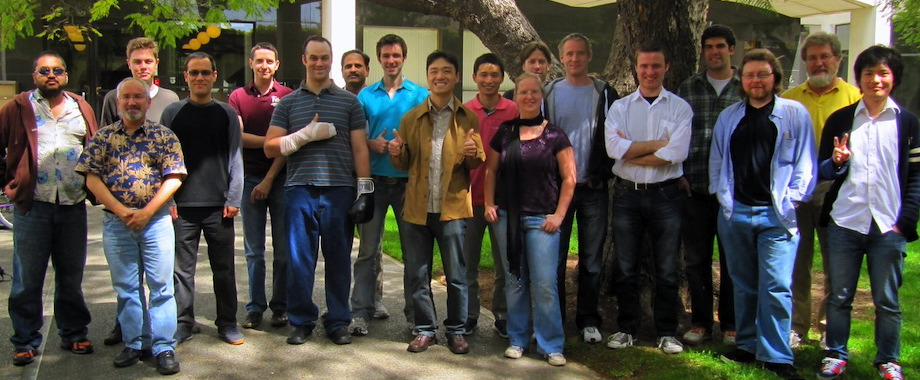
\includegraphics[width=6in]{LIGOX_29March2011.jpg}
\caption{LIGOX - The LIGO Instrument Science Group at Caltech.}
\label{fig:FigureKeyWord}
\end{center}
\end{figure}         


\begin{thebibliography}{9}
      
	\bibitem{CitationKeyWord}
	  Author,
	  \emph{Title of the Article or Book}.
	 Physical Review XXXX, XXXXX (2010).    
      
       \bibitem{URLsource}
       \url{http://blue.ligo-wa.caltech.edu:8000/40m/40mHomePage}
 
\end{thebibliography} %Must end the environment



\end{document} 
